% Lecture Template for ME3050 - Dynamic Modeling and Controls - Tennessee Technological University
% Spring 2024 - condensing and streamlining lectures by combining topics into a single PDF under the module name
% this will simplify file and link management as well as make lectures easier to use in class
% - added image/ to clean directory and reduce redundancy, specific to module for now  

% Module Name: - Automatic Control
% Topic 1 - Introduction to Control Systems
% Topic 2 - Control of First Order Plants
% Topic 3 - Control of Second Order Plants
% Topic 4 - Application and Implementation

\documentclass[fleqn]{beamer} % for presentation (has nav buttons at bottom)

%\usepackage{/home/tntech.edu/thill/courses/dmc/lectures/dmc_lectures}
\usepackage{/home/thill/courses/dmc/lectures/dmc_lectures}
%\usepackage{/mnt/c/Users/thill/Documents/courses/dmc/lectures/dmc_lectures}

\author{ME3050 - Dynamics Modeling and Controls}

\newcommand{\MNUM}{2\hspace{2mm}} % module number 
\newcommand{\moduletitle}{Automatic Control}

\newcommand{\sectionItitle}{Introduction to Control Systems}
\newcommand{\sectionIItitle}{Control of First Order Plants}
\newcommand{\sectionIIItitle}{Control of Second Order Plants}
\newcommand{\sectionIVtitle}{Application and Implementation}

\newcommand{\sectionIsubsectionItitle}{Open-Loop and Closed-Loop Control}
\newcommand{\sectionIsubsectionIItitle}{Control System Terminology}
\newcommand{\sectionIsubsectionIIItitle}{Modeling and Analysis}
\newcommand{\sectionIsubsectionIVtitle}{The PID Control Algorithm}

\newcommand{\sectionIIsubsectionItitle}{Block Diagram of Controlled System}
\newcommand{\sectionIIsubsectionIItitle}{DC Motor Example}
\newcommand{\sectionIIsubsectionIIItitle}{Simulation with Simulink}
\newcommand{\sectionIIsubsectionIVtitle}{Simulation with Simulink + Simscape}

\newcommand{\sectionIIIsubsectionItitle}{---}
\newcommand{\sectionIIIsubsectionIItitle}{---}
\newcommand{\sectionIIIsubsectionIIItitle}{---}
\newcommand{\sectionIIIsubsectionIVtitle}{---}

\newcommand{\sectionIVsubsectionItitle}{---}
\newcommand{\sectionIVsubsectionIItitle}{---}
\newcommand{\sectionIVsubsectionIIItitle}{---}
\newcommand{\sectionIVsubsectionIVtitle}{---}

\newcommand{\LT}{\mathcal{L}} % lagrangian

% custom box
\newsavebox{\mybox}

\title{Lecture Module - \moduletitle}

\date{Mechanical Engineering\vspc Tennessee Technological University}

\begin{document}

	\lstset{language=MATLAB,basicstyle=\ttfamily\small,showstringspaces=false}

	\frame{\titlepage \center\begin{framed}\Large \textbf{\moduletitle}\end{framed} \vspace{5mm}}

	% Module Outline
	\begin{frame} 
		\large \textbf{Lecture Module - \moduletitle} \vspace{3mm}\\

		\begin{itemize}
			\item Topic 1 - \hyperlink{sectionI}{\sectionItitle} \vspc % section I
			\item Topic 2 - \hyperlink{sectionII}{\sectionIItitle} \vspc % section II
			\item Topic 3 - \hyperlink{sectionIII}{\sectionIIItitle} \vspc % section III
			\item Topic 4 - \hyperlink{sectionIV}{\sectionIVtitle} \vspc % section IV
		\end{itemize}

	\end{frame}

	% section I
	\section{\sectionItitle}\label{sectionI}

		% section I Outline
		\begin{frame} 
			\large \textbf{Topic 1 - \sectionItitle} \vspace{3mm}\\

			\begin{itemize}
				\item \hyperlink{sectionIsubsectionI}{\sectionIsubsectionItitle} \vspc %  section I subsection I
				\item \hyperlink{sectionIsubsectionII}{\sectionIsubsectionIItitle} \vspc % section I subsection II
				\item \hyperlink{sectionIsubsectionIII}{\sectionIsubsectionIIItitle} \vspc % section I subsection III
				\item \hyperlink{sectionIsubsectionIV}{\sectionIsubsectionIVtitle} \vspc % section I subsection IV
			\end{itemize}
		\end{frame}
		
		% section I subsection I 
		\subsection{\sectionIsubsectionItitle}\label{sectionIsubsectionI}

			\begin{frame}
				\frametitle{\sectionIsubsectionItitle}
				\bigskip

				\textbf{Block Diagrams and Transfer Functions} 

				\vspace*{5mm}
				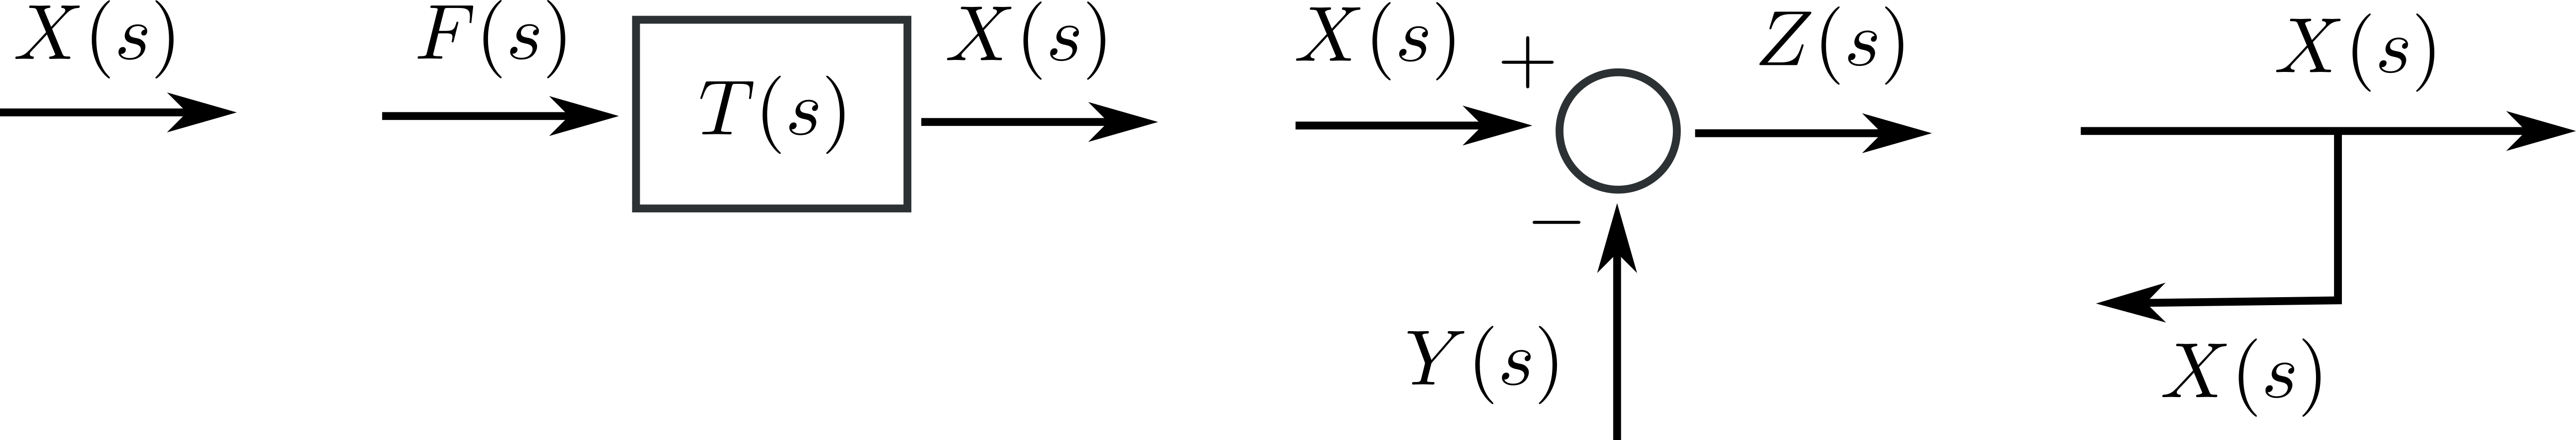
\includegraphics[scale=0.04]{images/four_basic_symbols.png}

				\begin{multicols}{2}
				\textbf{Generalized Feedback Loop}

				\vspace*{5mm}
				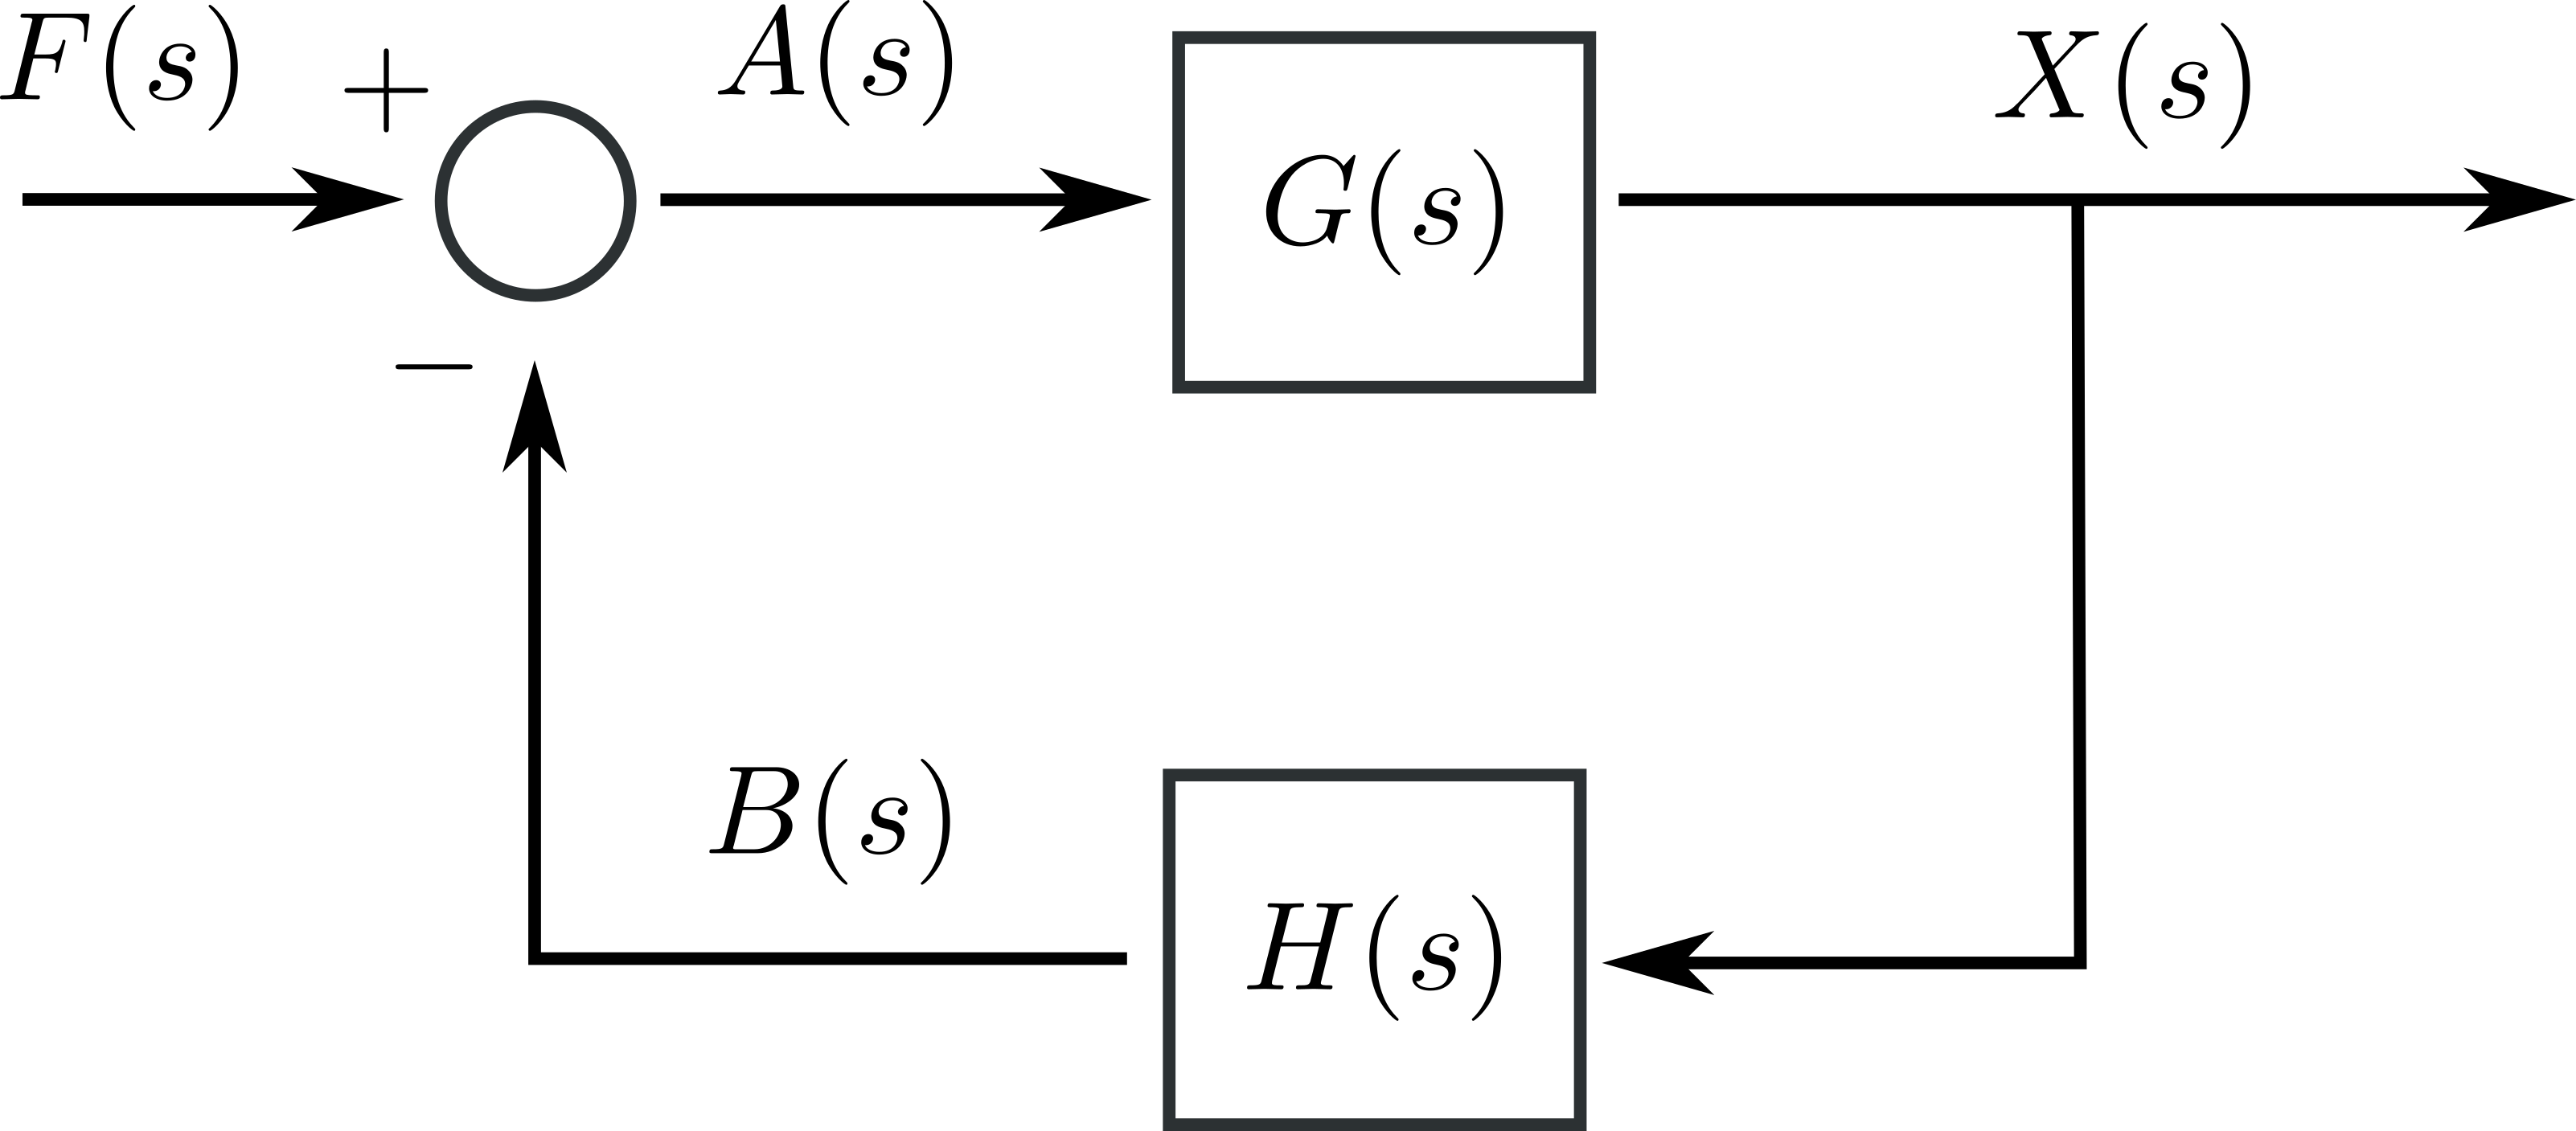
\includegraphics[scale=0.03]{images/generalized_feedback_loop.png}

				\[ T(s)=\frac{X(s)}{F(s)}\]

				\[ T(s)=\frac{G(S)}{1+G(s)H(s)}\]
				\end{multicols}

				\btVFill
			\end{frame}

			\begin{frame} \small
				\frametitle{\sectionIsubsectionItitle} 
				\bigskip

				\textbf{Control System Examples:}
                \begin{itemize}

                    \item Thermal Control - HVAC - 3D Printing
                    \item Vehicle Control - Cruise - ACC
                    \item Precision Motion Control - Robotics - Automation  

                \end{itemize}                   

                \vspace*{5mm}
                \textbf{Goal:} cause system {\it output} to go to specfied state

                \vspace*{5mm}
                \textbf{Strategy:} set the system input to appropriate value to do so
                \begin{itemize}
                	\item No Control 
                	\item Bang-Bang Control
                	\item Open-Loop Control
                	\item Closed-Loop Control
                \end{itemize}

				\btVFill
			\end{frame}

			\begin{frame}
				\frametitle{\sectionIsubsectionItitle}
				\bigskip

				\textbf{Open-Loop Control}
				\begin{itemize}

					\item uses prediction of model behavior, not system state

					\item less complex, known as {\it sensorless} 

					\item less robust to input disturbances

					\item single path block diagram

				\end{itemize}

				\vspace*{5mm}
				\textbf{Closed-Loop Control}
				\begin{itemize}

					\item uses measurement or estimation of model state and behavior

					\item more complex, requires integrated sensor

					\item can be robust to range of input disturbances 

					\item feedback loop in block diagram

				\end{itemize}

 
				\btVFill
			\end{frame}

				\begin{frame}\small
				\frametitle{\sectionIsubsectionItitle}
				\bigskip

				\textbf{Open-Loop Control}
				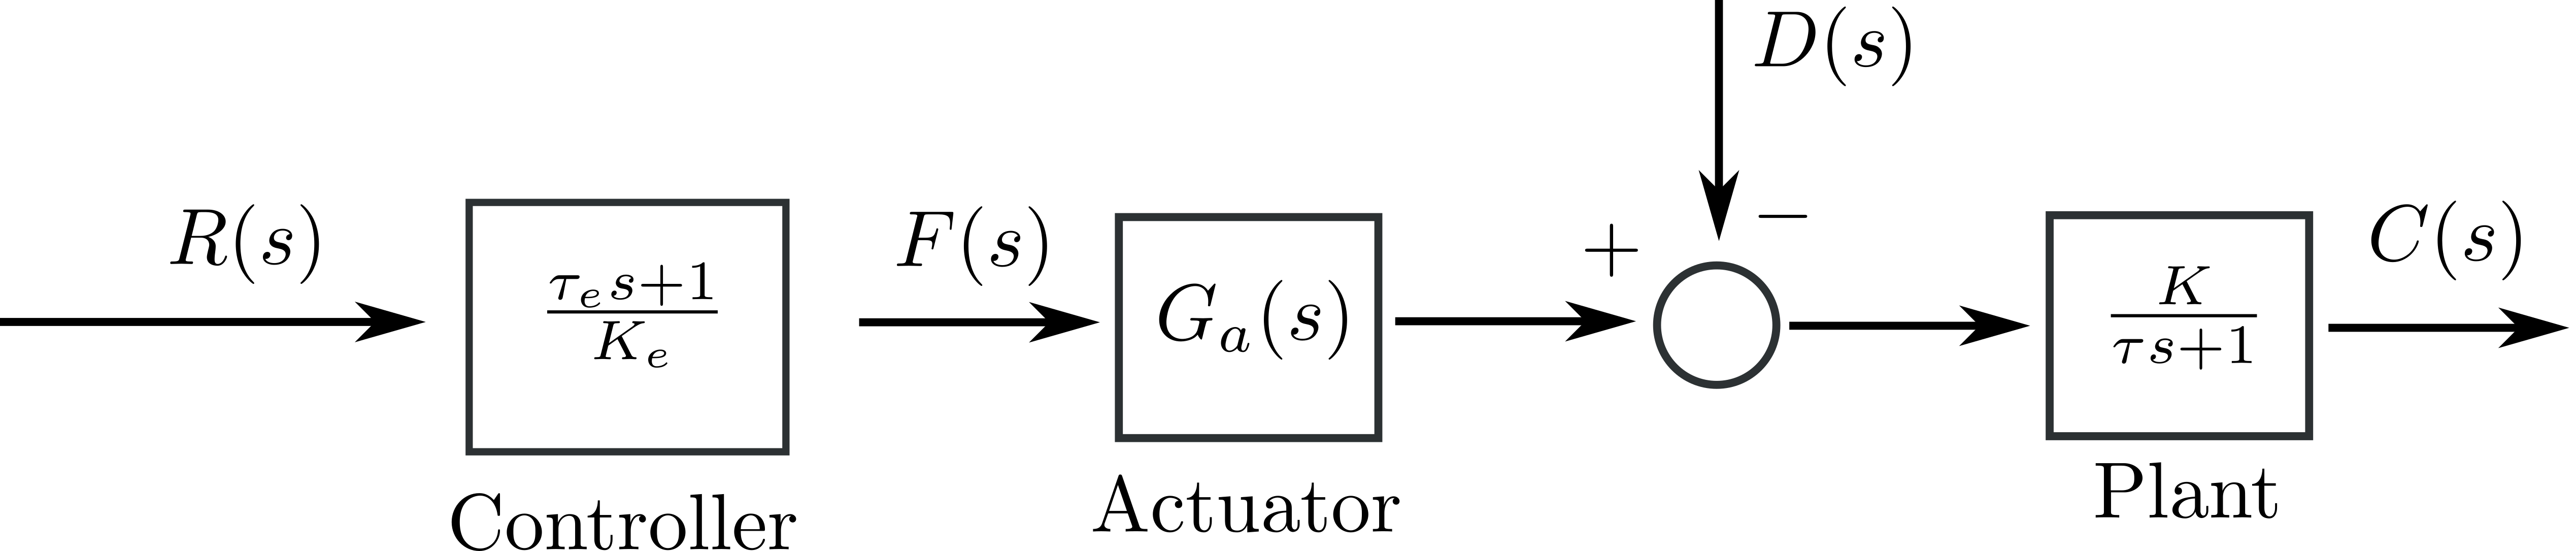
\includegraphics[scale=0.03]{images/open_loop_control.png}
				
				\vspace*{5mm}
				\textbf{Closed-Loop Control}
				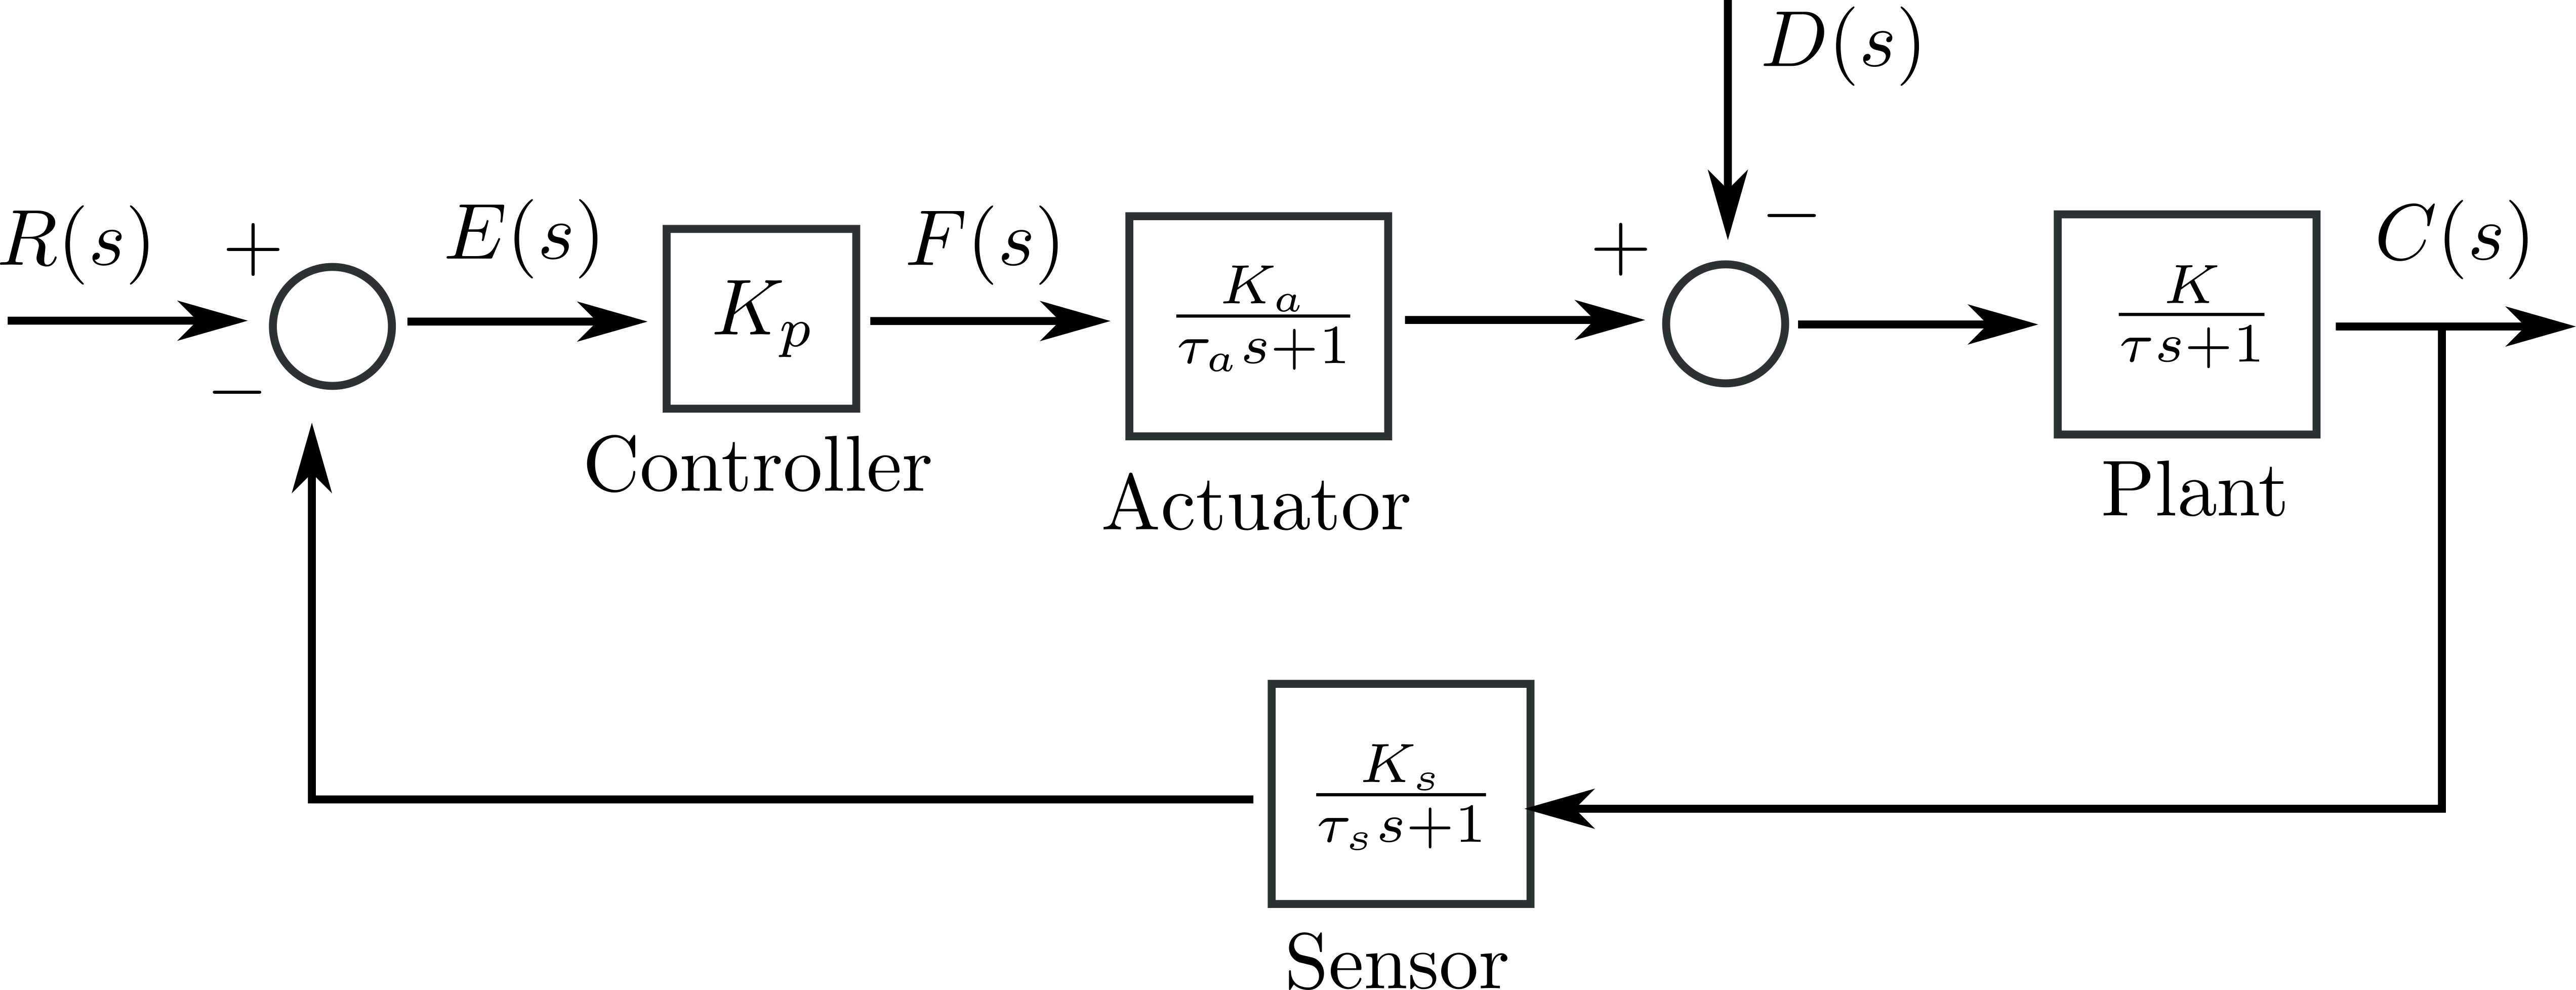
\includegraphics[scale=0.03]{images/closed_loop_control.png}
				
				\btVFill
				{\tiny images: T.Hill - modified from System Dynamics, Palm 3rd Ed.}
			\end{frame}

			

	
		% section I subsection II
		\subsection{\sectionIsubsectionIItitle}\label{sectionIsubsectionII}

			\begin{frame}
				\frametitle{\sectionIsubsectionIItitle}
				\bigskip

				\textbf{Closed-Loop Control Terminology}
				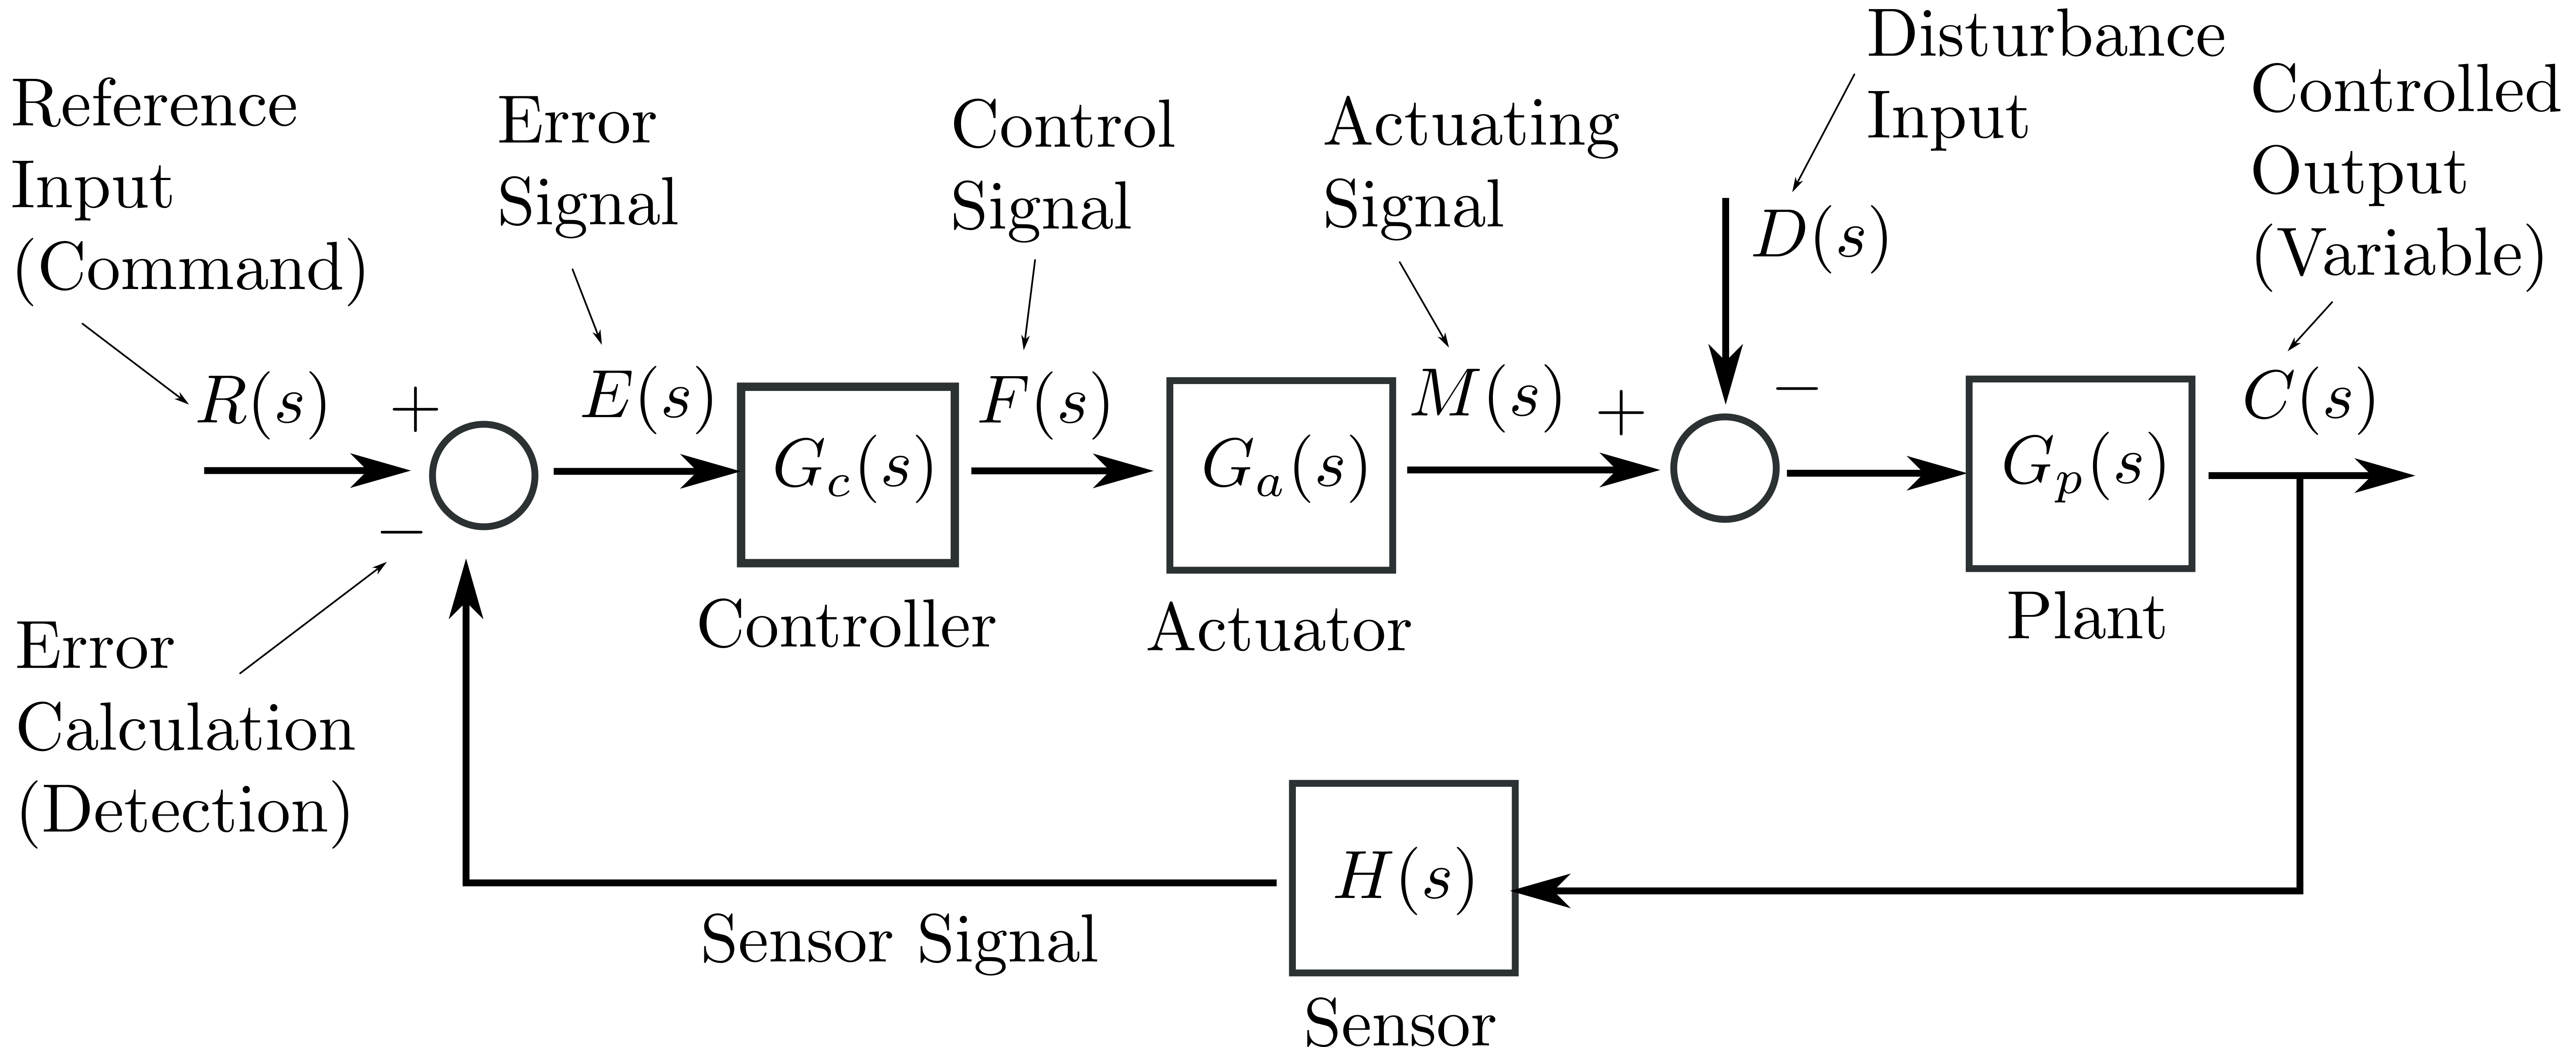
\includegraphics[scale=0.0375]{images/closed_loop_control_terminology.png}

				\btVFill
				{\tiny images: T.Hill - modified from System Dynamics, Palm 3rd Ed.}
			\end{frame}

				%\btVFill
			\begin{frame}
				\frametitle{\sectionIsubsectionIItitle}
				\bigskip

				
				\btVFill
			\end{frame}

		% section I subsection III
		\subsection{\sectionIsubsectionIIItitle}\label{sectionIsubsectionIII}
			\begin{frame} 
				\frametitle{\sectionIsubsectionIIItitle}
				\bigskip

				\btVFill
			\end{frame}	

			\begin{frame} 
				\frametitle{\sectionIsubsectionIIItitle}
				\bigskip

				\btVFill
			\end{frame}	

		% section I subsection IV
		\subsection{\sectionIsubsectionIVtitle}\label{sectionIsubsectionIV}

			\begin{frame}
				\frametitle{\sectionIsubsectionIVtitle}
				\bigskip

				The goal of the controller is to achieve the following:
				\begin{itemize}

					\item Minimize the steady state error
					\item Minimize the settling time
					\item Achieve other transient specifications (see time response)

				\end{itemize}

				\btVFill
				{\tiny Text: System Dynamics - Palm 3rd.}

			\end{frame}	

			\begin{frame}
				\frametitle{\sectionIsubsectionIVtitle}
				\bigskip

				\textbf{The PID Control Algorithm}
				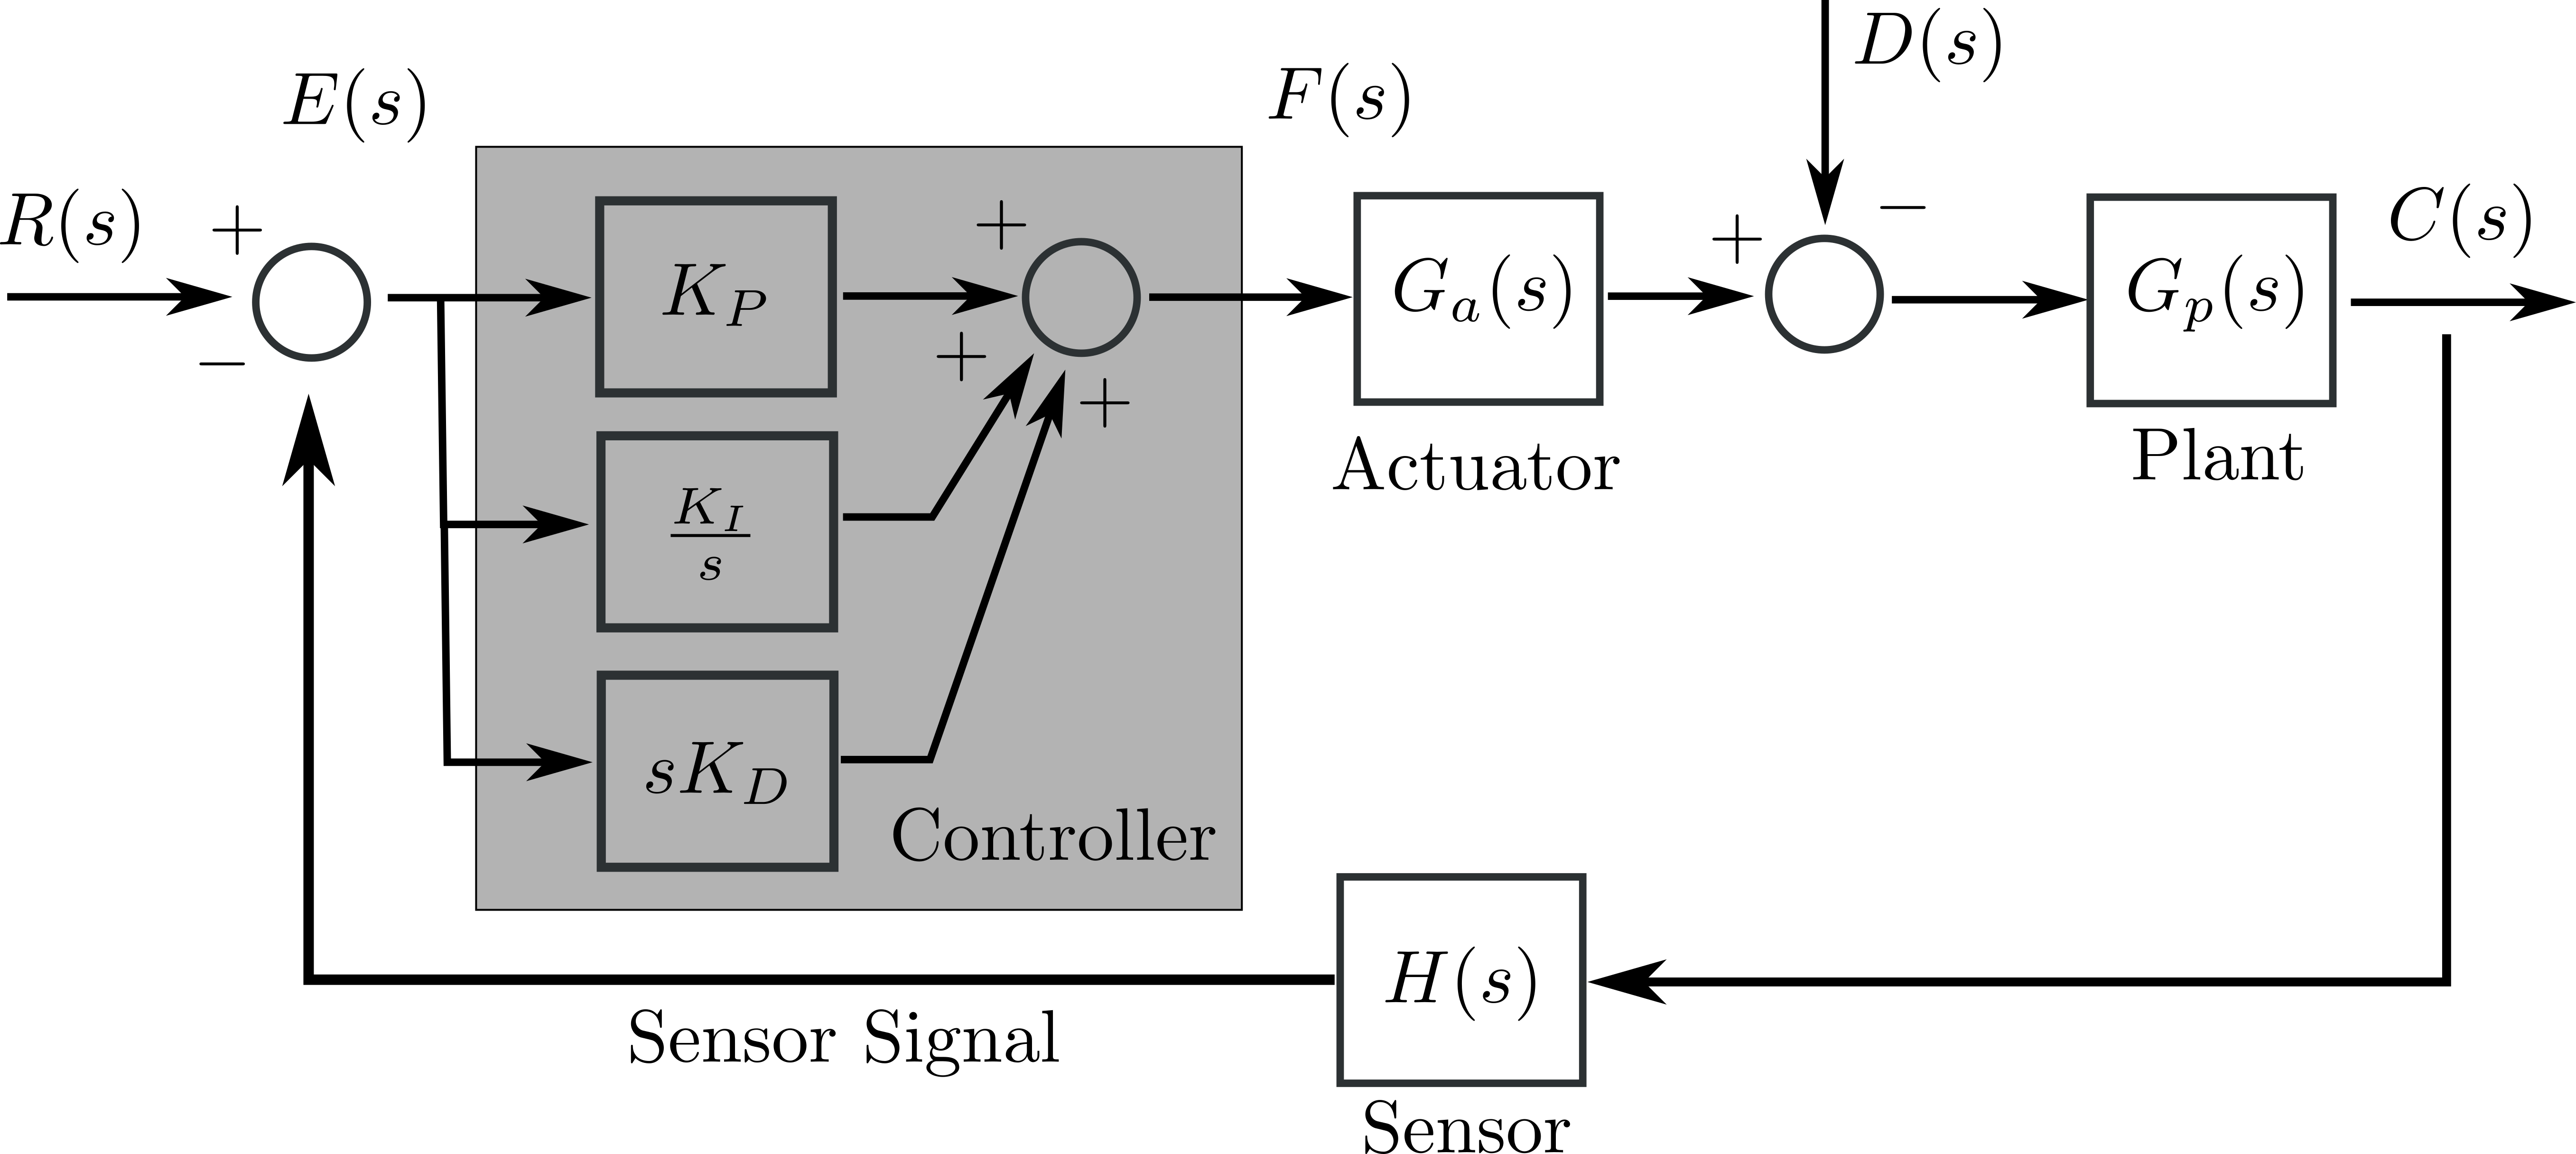
\includegraphics[scale=0.0375]{images/closed_loop_control_pid.png}

				\btVFill
			\end{frame}	

			\begin{frame}
				\frametitle{\sectionIsubsectionIVtitle}
				\bigskip

				The {\textbf control gains} scale the calculated error to adjust the system input(s).

				\vspace*{5mm}
				\begin{itemize}

					\item $K_P$ - {\it Proportional} Gain - Correction from current error \vspace*{5mm}
					\item $K_I$ - {\it Integral} Gain - Correction from acculated error \vspace*{5mm}
 					\item $K_D$ - {\it Derivative} Gain - Correction from change in error \vspace*{5mm}

				\end{itemize}

				Note: P, PI, and PD controllers can be used, but the combination PID is prefered. 
				

				\btVFill
			\end{frame}

			\begin{frame}
				\frametitle{\sectionIsubsectionIVtitle}
				\bigskip

				\frametitle{References}

				\begin{itemize}
					\item System Dynamics, Palm III, Third Edition - Chapter 10 - Introduction to Feedback Control Systems
				\end{itemize}
			
				\btVFill
			\end{frame}
	
	% Section II
	\section{\sectionIItitle}\label{sectionII}

		% section II Outline
		\begin{frame}
			\large \textbf{Topic 2 - \sectionIItitle} \vspace{3mm}\\

			\begin{itemize}
				\item \hyperlink{sectionIIsubsectionI}{\sectionIIsubsectionItitle} \vspc %  section II subsection I
				\item \hyperlink{sectionIIsubsectionII}{\sectionIIsubsectionIItitle} \vspc % section II subsection II
				\item \hyperlink{sectionIIsubsectionIII}{\sectionIIsubsectionIIItitle} \vspc % section II subsection III
				\item \hyperlink{sectionIIsubsectionIV}{\sectionIIsubsectionIVtitle} \vspc % section II subsection IV
			\end{itemize}

		\end{frame}

		% section II subsection I
		\subsection{\sectionIIsubsectionItitle}\label{sectionIIsubsectionI}

			\begin{frame}[label=sectionIIsubsectionI]
				\frametitle{\sectionIIsubsectionItitle}
				\bigskip

				\frametitle{Harmonic Input Function}
				
				\btVFill
			\end{frame}

			\begin{frame}[label=sectionIIsubsectionI]
				\frametitle{\sectionIIsubsectionItitle}
				\bigskip

				\btVFill
			\end{frame}

			\begin{frame}[label=sectionIIsubsectionI]
				\frametitle{\sectionIIsubsectionItitle}
				\bigskip

				\btVFill
			\end{frame}


		% section II subsection II
		\subsection{\sectionIIsubsectionIItitle}\label{sectionIIsubsectionII}

			\begin{frame}

				\frametitle{\sectionIIsubsectionIItitle}
				\bigskip

				\btVFill 
			\end{frame}

			\begin{frame}

				\frametitle{\sectionIIsubsectionIItitle}
				\bigskip

				\btVFill 
			\end{frame}




		% section II subsection III
		\subsection{\sectionIIsubsectionIIItitle}\label{sectionIIsubsectionIII}

			\begin{frame}
				\frametitle{\sectionIIsubsectionIIItitle}
				\bigskip


				\btVFill 
			\end{frame}	


			\begin{frame}
				\frametitle{\sectionIIsubsectionIItitle}
				\bigskip
								
				\btVFill 
			\end{frame}	


			\begin{frame}
				\frametitle{\sectionIIsubsectionIIItitle}
				\bigskip

				
				\btVFill 
			\end{frame}

			\begin{frame}
				\frametitle{\sectionIIsubsectionIIItitle}
				\bigskip

								
				\btVFill 
			\end{frame}

			\begin{frame}
				\frametitle{\sectionIIsubsectionIIItitle}
				\bigskip

				
				\btVFill 
			\end{frame}

			
		% section II subsection IV
		\subsection{\sectionIIsubsectionIVtitle}\label{sectionIIsubsectionIV}

			\begin{frame}[containsverbatim]
				\frametitle{\sectionIIsubsectionIVtitle}
				\bigskip

								
				\btVFill 
			\end{frame}	

			\begin{frame}
				\frametitle{\sectionIIsubsectionIVtitle}
				\bigskip


				\btVFill 
			\end{frame}	
		
	% Section III
	\section{\sectionIIItitle}\label{sectionIII}

		% section III Outline
		\begin{frame}
			\large \textbf{Topic 3 - \sectionIIItitle} \vspace{3mm}\\

			\begin{itemize}
				\item \hyperlink{sectionIIIsubsectionI}{\sectionIIIsubsectionItitle} \vspc %  section III subsection I
				\item \hyperlink{sectionIIIsubsectionII}{\sectionIIIsubsectionIItitle} \vspc % section III subsection II
				\item \hyperlink{sectionIIIsubsectionIII}{\sectionIIIsubsectionIIItitle} \vspc % section III subsection III
				\item \hyperlink{sectionIIIsubsectionIV}{\sectionIIIsubsectionIVtitle} \vspc % section III subsection IV
			\end{itemize}

		\end{frame}

		% section III subsection I
		\subsection{\sectionIIIsubsectionItitle}\label{sectionIIIsubsectionI}

			\begin{frame}
				\frametitle{\sectionIIIsubsectionItitle}
				\bigskip


				\btVFill
			\end{frame}

			\begin{frame}
				\frametitle{\sectionIIIsubsectionItitle}
				\bigskip

				\btVFill
			\end{frame}

		% section III subsection II
		\subsection{\sectionIIIsubsectionIItitle}\label{sectionIIIsubsectionII}	

			\begin{frame}
				\frametitle{\sectionIIIsubsectionIItitle}
				\bigskip


				\btVFill
			\end{frame}

			\begin{frame}
				\frametitle{\sectionIIIsubsectionIItitle}
				\bigskip


				\btVFill
			\end{frame}

		% section III subsection III
		\subsection{\sectionIIIsubsectionIIItitle}\label{sectionIIIsubsectionIII}

			\begin{frame}
				\frametitle{\sectionIIIsubsectionIIItitle}
				\bigskip

	
				\btVFill
			\end{frame}

			\begin{frame}
				\frametitle{\sectionIIIsubsectionIIItitle}
				\bigskip

				\btVFill
			\end{frame}

			\begin{frame}
				\frametitle{\sectionIIIsubsectionIIItitle}
				\bigskip

				\btVFill
			\end{frame}

		% section III subsection IV
		\subsection{\sectionIIIsubsectionIVtitle}\label{sectionIIIsubsectionIV}	

			\begin{frame}[containsverbatim]
				\frametitle{\sectionIIIsubsectionIVtitle}
				\bigskip
				\btVFill 
			\end{frame}

			\begin{frame}
				\frametitle{\sectionIIIsubsectionIVtitle}
				\bigskip

		 		\btVFill 
			\end{frame}

	% Section IV
	\section{\sectionIVtitle}\label{sectionIV}

		% section IV Outline
		\begin{frame}
			\large \textbf{Topic 3 - \sectionIVtitle} \vspace{3mm}\\

			\begin{itemize}
				\item \hyperlink{sectionIVsubsectionI}{\sectionIVsubsectionItitle} \vspc %  section III subsection I
				\item \hyperlink{sectionIVsubsectionII}{\sectionIVsubsectionIItitle} \vspc % section III subsection II
				\item \hyperlink{sectionIVsubsectionIII}{\sectionIVsubsectionIIItitle} \vspc % section III subsection III
				\item \hyperlink{sectionIVsubsectionIV}{\sectionIVsubsectionIVtitle} \vspc % section III subsection IV

			\end{itemize}

		\end{frame}

		% section IV subsection I
		\subsection{\sectionIVsubsectionItitle}\label{sectionIVsubsectionI}

			\begin{frame}
				\frametitle{\sectionIVsubsectionItitle}
				\bigskip

				\btVFill
			\end{frame}

			\begin{frame}
				\frametitle{\sectionIVsubsectionItitle}
				\bigskip
				
				\btVFill
			\end{frame}

		% section IV subsection II
		\subsection{\sectionIVsubsectionIItitle}\label{sectionIVsubsectionII}	

			\begin{frame}
				\frametitle{\sectionIVsubsectionIItitle}
				\bigskip
	
				\btVFill
			\end{frame}

			\begin{frame}
				\frametitle{\sectionIVsubsectionIItitle}
				\bigskip

	
				\btVFill
			\end{frame}

			\begin{frame}
				\frametitle{\sectionIVsubsectionIItitle}
				\bigskip

	
				\btVFill
			\end{frame}

		% section IV subsection III
		\subsection{\sectionIVsubsectionIIItitle}\label{sectionIVsubsectionIV}

			\begin{frame}
				\frametitle{\sectionIVsubsectionIIItitle}
				\bigskip

	
			
				\btVFill
			\end{frame}

			\begin{frame}
				\frametitle{\sectionIVsubsectionIIItitle}
				\bigskip

				\btVFill
			\end{frame}

			\begin{frame}
				\frametitle{\sectionIVsubsectionIIItitle}
				\bigskip

				\btVFill
			\end{frame}

			\begin{frame}
				\frametitle{\sectionIVsubsectionIIItitle}
				\bigskip

				\btVFill
			\end{frame}

			\begin{frame}
				\frametitle{\sectionIVsubsectionIIItitle}
				\bigskip


				\btVFill
			\end{frame}

		% section IV subsection IV
		\subsection{\sectionIVsubsectionIVtitle}\label{sectionIVsubsectionIV}	

			\begin{frame}
				\frametitle{\sectionIVsubsectionIVtitle}
				\bigskip



				

				\btVFill 
			\end{frame}

			\begin{frame}
				\frametitle{\sectionIVsubsectionIVtitle}
				\bigskip

			

		 		\btVFill 
			\end{frame}
			
			\begin{frame}
				\frametitle{\sectionIVsubsectionIVtitle}
				\bigskip
				
				
					
				\btVFill 
			\end{frame}

			\begin{frame}
				\frametitle{\sectionIVsubsectionIVtitle}
				\bigskip
			
				
				\btVFill 
			\end{frame}



\end{document}





